\documentclass[tikz]{standalone}

\usetikzlibrary{fit}
\usetikzlibrary{shapes,arrows}
\usetikzlibrary {shapes.misc} 
\usetikzlibrary{arrows.meta}
\usetikzlibrary{calc,positioning}
\usetikzlibrary{patterns,decorations.pathmorphing,decorations.markings}

\begin{document}
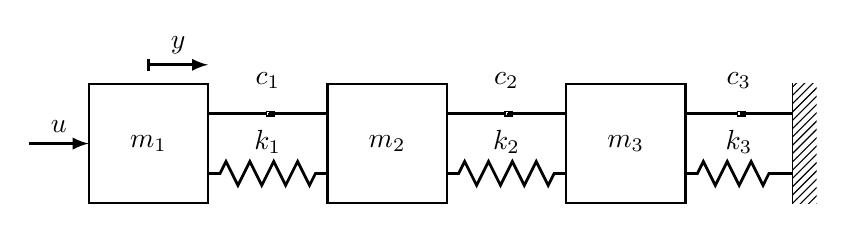
\begin{tikzpicture}
    \def\massWidth{0.125\linewidth}
    \def\massHeight{\massWidth}
    \def\massDistance{\massWidth}
    \def\scale{0.1}

    \tikzstyle{spring}=[line width=1pt,decorate,decoration={zigzag,pre length=0.1*\massDistance,post
    length=0.1*\massDistance,segment length=0.2*\massDistance, amplitude=0.1*\massHeight}]
    
    \tikzstyle{damper}=[line width=1pt,decoration={markings,  
      mark connection node=dmp,
      mark=at position 0.5 with 
      {
        \node (dmp) [line width=0.5pt,inner sep=0pt,transform shape,rotate=-90,minimum
    width=\scale*0.25*\massHeight,minimum height=\scale*0.125*\massWidth,draw=none] {};
        \draw [line width=0.5pt] ($(dmp.north east)+(2pt,0)$) -- (dmp.south east) -- (dmp.south
    west) -- ($(dmp.north west)+(2pt,0)$);
        \draw [line width=0.5pt] ($(dmp.north)+(0,\scale*-0.08*\massHeight)$) -- ($(dmp.north)+(0,\scale*0.08*\massHeight)$);
      }
    }, decorate]
    
    \tikzstyle{ground}=[fill,pattern=north east lines,draw=none,minimum
    width=0.75cm,minimum height=0.3cm]

    \tikzstyle{wall}=[fill,pattern=north east lines,draw=none,minimum
    width=0.3cm,minimum height=0.7cm]
    
    % Masses
    \node[draw,outer sep=0pt,thick] (M1) [minimum width=\massWidth, minimum height=\massHeight] {$m_1$};
    \node[draw,outer sep=0pt,thick] (M2) at (\massWidth + \massDistance,0) [minimum width=\massWidth, minimum height=\massHeight] {$m_2$};
    \node[draw,outer sep=0pt,thick] (M3) at (2*\massWidth + 2*\massDistance,0) [minimum width=\massWidth, minimum height=\massHeight] {$m_3$};
    % \node (dots) at (2*\massWidth + 1.625*\massDistance,0) {$\scriptstyle\cdots$};
    
    % Support
    \node[wall, minimum height=\massHeight] (support) at (3*\massWidth + 2.5*\massDistance,0) {};
    \draw (support.north west) -- (support.south west);
    
    % Springs and Dampers
    \draw[spring] ($(M1.east) - (0,0.25*\massHeight)$) -- ($(M2.west) - (0,0.25*\massHeight)$) 
    node [midway,above, yshift=0.08*\massHeight] {$k_1$};
    \draw[damper] ($(M1.east) + (0,0.25*\massHeight)$) -- ($(M2.west) + (0,0.25*\massHeight)$)
    node [midway,above, yshift=0.12*\massHeight] {$c_1$};
    \draw[spring] ($(M2.east) - (0,0.25*\massHeight)$) -- ($(M3.west) - (0.0*\massWidth,0.25*\massHeight)$) 
    node [midway,above, yshift=0.08*\massHeight] {$k_2$};
    \draw[damper] ($(M2.east) + (0,0.25*\massHeight)$) -- ($(M3.west) + (-0.0*\massWidth,0.25*\massHeight)$)
    node [midway,above, yshift=0.12*\massHeight] {$c_2$};
    \draw[spring] ($(M3.east) - (0,0.25*\massHeight)$) -- ($(support.west) - (0.0,0.25*\massHeight)$) 
    node [midway,above, yshift=0.08*\massHeight] {$k_3$};
    \draw[damper] ($(M3.east) + (0,0.25*\massHeight)$) -- ($(support.west) + (-0.0,0.25*\massHeight)$)
    node [midway,above, yshift=0.12*\massHeight] {$c_3$};
    
    \draw[-latex, line width=1pt] ($(M1.west) - (0.5*\massWidth,0)$) -- ($(M1.west)$) node [midway, above] {$u$};

    \draw[-latex, line width=1pt] ($(M1.east) - (0.5*\massWidth, -0.66 * \massHeight)$) -- ($(M1.east) + (0, 0.66 * \massHeight)$) node [midway, above] {$y$};

    \draw[line width =1pt] ($(M1.east) - (0.5*\massWidth, -0.61 * \massHeight)$) -- ($(M1.east) - (0.5*\massWidth, -0.71 * \massHeight)$);
\end{tikzpicture}
\end{document}